\documentclass[]{report}
\usepackage{graphicx}
\usepackage{todonotes}	
\usepackage{booktabs}
\usepackage{listings}
\usepackage[margin=1in]{geometry}
\usepackage{float}
\graphicspath{{resources/images/}}
\setcounter{secnumdepth}{5}



% Title Page
\title{Utilising peer-to-peer networking for data transfer over the browser}
\author{Dominic Rathbone \\ Student Number: 12843140 \\ BSc Computer Science}


\begin{document}
\maketitle
\tableofcontents

\chapter{Project Scope}
\section{Aims and Objectives}
	The ultimate objective of my project is to investigate the plausibility of data transfer over web browsers (in particular, with file transfer and media streaming) without the need for a centralised client-server architecture, instead opting for a peer-to-peer network architecture. In order to do so, I plan to:
	\begin{itemize}
		\item Research peer-to-peer networking architecture and topologies
		\item Research WebRTC
		\item Research signalling protocols
		\item Research media streaming compression \& protocols
		\item Research client-side JavaScript frameworks
		\item Develop a session signalling server in Java with the WebSockets protocol
		\item Develop a WebRTC Application to transfer and stream uploaded files.
		\item Implement a structured peer to peer network between peers transferring/streaming a file using the web application.
	\end{itemize}
\section{Stakeholders}
	The stakeholders involved in my project will be myself, my supervisor, Stelios Kapetanakis and the user.
\section{Methods of Communication}
	Stelios and I have set up a regular meeting once a week on Friday at 4pm to catch up. On top of this, we communicate regularly via email and Stelios has access to a project git repository on GitHub and a workflow board set up on my web server to track the progress of my project. 
	
\chapter{Research}
\section{Comparing Network Architectures}	
	Peer-to-peer networking is the distribution of resources and processing between the nodes of a network. These networks tend to take the form of an overlay network which is a topology describing a virtual network that sits on top of a physical network (e.g the internet) consisting of a subset of the nodes connected to the physical network.
	
	\begin{figure}[H]
		\caption{
			An Unstructured Peer-To-Peer Overlay Network 	
			\cite{Unstructured P2P Diagram}
		}
		\centering
		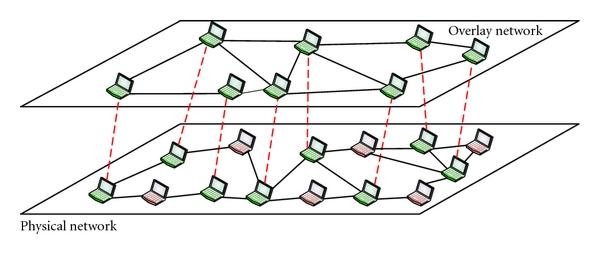
\includegraphics{overlaynetwork.jpg}
	\end{figure}
	
	Although an overlay network does not need to manage the burden the physical network is responsible for, in order to discover and route new nodes, it needs to have some way of managing the subset of nodes using it. There are several different ways of defining how it does this:
	
	\begin{itemize}
		\item Unstructured peer-to-peer:
		Peer connections in the overlay are established randomly and do not adhere to a network topology. New peers copy the connections another peer has formed and develops it's own over time.\cite{P2P overlay networks}. These networks are easier to build than structured networks as routing is random and they also tend to fair better in periods when the rate of peers leaving and joining (churn rate) is high due to their non-deterministic nature. However, searching in these networks tends to be less efficient as they rely on flooding the network to find nodes that have the data they are searching for.
		\item Structured peer-to-peer:
		Peers in a network are organised in a specified network topology and generally use a distributed hash table (DHT) to link together. The DHT consists of many peers maintaining a partial hash table referencing the unique keys of other peers in the network, allowing it to route to them. This way, a peer can communicate with another by hopping messages through peers in their hash table. Generally, each peer's hash table consists of nodes getting exponentially further away from it in order to improve the efficiency of this process. \cite{P2P overlay networks}. 
		\item Hybrid peer-to-peer:
		A combination of  peer-to-peer and client-server models, these networks use centralized servers in some way.  This model tends to work better than both unstructured and structured as dependent on how it is implemented, features that function better in decentralized networks can be left to the peers in network whilst the server can handle the features it is better at. \cite{Hybrid P2P network}
	\end{itemize}
				
	Additionally, there is also the client-server model. In a basic sense, this is when the machines processing data (servers) are distinct from the computers requesting this processing (client), although in actuality, the boundaries between them vary dependent on how it is implemented. Whilst the shift of processing on to the service supplier means that the user of the application does not need a powerful machine to run it, it also means that the service supplier has the responsibility of maintaining and paying for these servers. Furthermore, although modern server architectures are designed in a distributed structure granting them to be more robust (as distribution allows for redundancy and load balancing), if these servers undergo too much load or in extreme cases, if the server farm completely crashes, the user would not be able to use the application as intended.
	
	Using a peer to peer architecture avoids the issues associated with the client-server model as processing is distributed between the nodes making up the network, resulting in it being cheaper to maintain as there is less reliance on servers and more robust as the network scales as load increases. However, there are a number of considerations to be aware of in peer to peer networking, the largest of which being security as there is no centralized authority to manage access control to resources. Thus, a malicious client could potentially launch a number of attacks versus other nodes in the network such as Denial Of Service (DoS) where a malicious group of nodes floods a network with a massive amount of fake data, potentially crashing nodes within it or Man in the Middle (MitM) attacks where a node is able to intercept data flowing between two other nodes and spy on or poison this data\cite{P2P Security Issues}. Whilst it would be hard to completely avoid risks like this as it is an inherent flaw in peer-to-peer architecture, introducing the basic concept of trust into a peer-to-peer network can stop malicious peers from entering it in the first place. This will be implemented in my application by allowing users to enable authentication (via password) for the uploaded file potentially preventing malicious attackers from being able to download or stream it. 
	
	My application will most closely resemble a hybrid peer-to-peer network as even though the actual channel for transferring data between peers (WebRTC Data Channel) will not go through a server, it will use a signalling server to route peers together. To form a network of peers that go beyond the one-to-many peer connection established by WebRTC, the signalling server in conjunction with the client-side application will have to manage how these peers connect to each other. A way of doing this is to connect new peers to the second newest peer and so on, forming a linear chain of peers that can reroute if the neighbouring peer disconnected.
	\begin{figure}[H]
		\centering
		\caption{Linear network}
		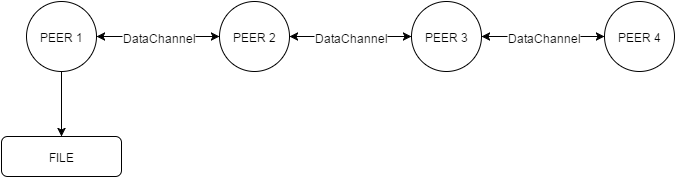
\includegraphics[scale=0.4]{network.png}
	\end{figure}
	\begin{figure}[H]
		\centering
		\caption{Peer disconnects from the network}
		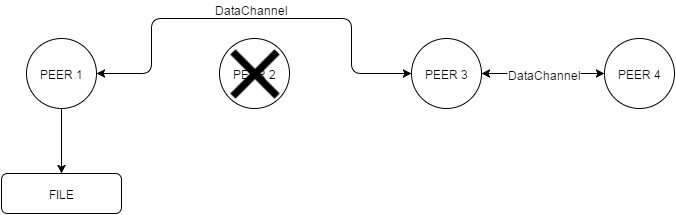
\includegraphics[scale=0.4]{peerdisconnect.png}
	\end{figure}
	However, this would prove inefficient if a peer in the chain malfunctioned or restricted bandwidth, potentially bottlenecking the rest of the peers behind it. As an alternative, peers could be routed based on a tree network topology \cite{Tree Topology} consisting of supernodes, "high capability" nodes that relay the transferred data to subnodes. This way load can be balanced across many nodes by distributing new nodes to another supernode or by electing further supernodes if it increases too much or if one disconnects. By exploiting heterogeneity between peers of the network, this topology can also be used to improve performance within the network by electing supernodes based on criteria such as location and, in our case, how much of the data has already been transferred or streamed to them. By doing so, performance within a network can potentially be improved as subnodes can be connected to supernodes based on this criteria, e.g if a subnode is located in the same place as a supernode then use it.\cite{Supernodes}.		
	\begin{figure}[H]
		\centering
		\caption{Tree Network}
		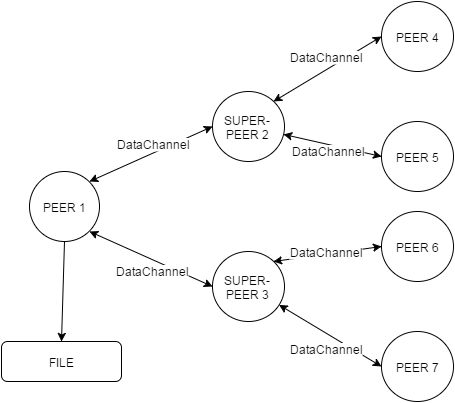
\includegraphics[scale=0.4]{treetopology.png}
	\end{figure}			
\section{Current Solutions to Data Transfer}
	Currently, solutions such as DropBox and Google Drive focus on cloud storage as a service whilst providing the ability to transfer data as a secondary function of this service. Although this is an extremely valuable and convenient idea enabling consumers to back-up their data, not all want a third party service that stores the data they want to transfer as this practice does raise ethical issues, namely with the data's security, privacy and ownership once it has been uploaded. However as a consumer, this can be hard to avoid when the online storage and transfer of data are so closely intertwined as these services have a huge market share.
	
	Once you have uploaded files to one of these services, there is a trust placed on the company to store the data securely. However you could argue that this trust is misplaced, in 2010, the "Cloud Security Alliance" released a regularly updated list of the top threats faced by cloud computing services submitting there are numerous security issues faced within the cloud computing industry with many of the issues on this list occurring due to malicious intentions. For example the 6th item on the list, "Malicious Insiders" describes a situation in which current or former employees abuse their authorizations within system to gain access to sensitive information \cite{CSA Top Threats}. This suggests that even though companies can protect their client's data to an extent, there are still issues the industry face that consumers may want to avoid.

 	Whilst the uploaded data can be encrypted in a way that means only clients of the service can decrypt it (through end-to-end encryption), many people feel insecure leaving traces of their private information on a remote server belonging to a company that is not necessarily always acting in their interest. In 2013, this concern was legitimized by Edward Snowden when he disclosed information about government surveillance programs such as PRISM that coerced firms such as Google, Microsoft and Yahoo to provide private consumer data from their services to the government.\cite{PRISM}  More recently, this idea has been reinforced by legislation such as the "Investigatory Powers Bill" being introduced in the UK that could prohibit companies from using end-to-end encryption techniques allowing authorities to request decrypted client data \cite{IPB Encryption}. Whilst we can assume they have done this with non-malicious intentions, by weakening the encryption practices of these companies, they will potentially weaken the defence against malicious attackers.
	
	As an alternative to using cloud storage solutions for sharing files, there is also specific data transfer sites such as WeTransfer that allows you to send files up to 2gb via their site. This works by sending a link through email to the person you want to send the file to. Whilst it does store the uploaded files, they are only kept for 7 days in order to prevent unnecessary storage costs \cite{WeTransfer Storage Time}. Although this is better for data privacy, WeTransfer use third party providers such as Amazon Web Services (AWS) to store this data using AWS S3 Storage \cite{WeTransfer AWS Case Study} meaning there is still the potential concern of data privacy and security highlighted previously.
	
	Peer-to-peer networks also been popular for file sharing since the late 1990s due to the rise of applications such as Napster which focused on peer to peer music sharing. Napster worked by using a central server to index files that each peer made available on their machine. Each peer would then be able to search the index for copies of songs and download them from each other. However, this service was eventually shut down as the company ran into legal problems with copyright infringement. Since then, protocols such as BitTorrent have improved on the idea of peer to peer sharing. The BitTorrent protocol works by peers creating ".torrent" descriptor files that describe the file's metadata, this is then shared however it is seen fit. Each peer wanting to download this file then picks up this ".torrent" file, opens it with a BitTorrent client and joins a "swarm" of peers, becoming one of the many "leechers" downloading this file. At the same time, this peer becomes one of the many "seeders" uploading this file as they download it so that other leechers can download it from them. The initial peer discovery is based on "trackers", servers hosting lists of seeders and leechers for the file. One of the issues with BitTorrent is that in order to share a file, you must go through the process of downloading a client, creating a ".torrent" file, adding it to a trackers list and sharing the ".torrent" with your peers and this can be seen as a arduous task for a basic consumer looking to share their files. Another problem is that if a tracker is compromised, there is potential for malicious attacks using the information stored on there.

	As an alternative to these current solutions, the application I plan to develop has the aim of separating the online transfer of data from it's storage by connecting the peers involved in the transfer directly with each other. This circumvents the problems with cloud storage as the data being transferred does not pass through any servers as well as the problems with current peer to peer file sharing as it does not require a desktop client or torrent files. To allow my application to share files online, WebRTC will be used.
	
\section{WebRTC}			
	WebRTC (Real Time Communication) is an emerging web technology that enables browsers to communicate real time via a peer-to-peer connection, avoiding the need for a centralized server to transfer data between clients. This was first released by Google as an open source project in May 2011 \cite{Google WebRTC Release} and was later drafted as an API definition by W3C remaining as a work in progress. \cite{W3C WebRTC Definition}. WebRTC has yet to be fully implemented in every web browser but Chrome, Firefox and a WebRTC specific browser called Bowser do support it. Firefox (Nightly), in particular seems to be leading the way in this so the application will specifically be developed towards this browser\cite{WebRTC browser support}.
	The 3 main WebRTC APIs supported at this time are:
		\begin{itemize}
			\item RTCDataChannel:
			"The RTCDataChannel interface represents a bi-directional data channel between two peers of a connection." \cite{Mozilla Web API}
			\item RTCPeerConnection:
			"The RTCPeerConnection interface represents a WebRTC connection between the local computer and a remote peer. It is used to handle efficient streaming of data between the two peers." 
			\cite{Mozilla Web API}
			\item getUserMedia:
			"Prompts the user for permission to use one video and/or one audio input device such as a camera or screensharing and/or a microphone. If the user provides permission, then the successCallback is invoked with the resulting MediaStream object as its argument. If the user denies permission or media is not available, then the errorCallback is called with PermissionDeniedError or NotFoundError respectively. Note that it is possible for neither completion callback to be called, as the user is not required to make a choice."\cite{Mozilla Web API}
		\end{itemize}
	In order to achieve it's aim, the application will utilize the RTCPeerConnection and RTCDataChannel APIs. The former to establish a peer connection between two clients and to stream whilst the latter will be used to create a data channel over this peer connection to transfer data.
			
	As mentioned in the Javascript Session Establishment Protocol (JSEP) \cite{JSEP}, although WebRTC and the browser is used to transfer the data between two peers, it purposely does not handle signalling. This is a concept that came from telecommunications and utilised in VoIP and is the process of organising the communication between two clients, handling the exchange of metadata that creates and manages a session. The rationale behind WebRTC being signalling protocol-agnostic is that different applications will require particular protocols in order to, for example, fit into previously existing architecture. In the case of my application, to handle signalling, Session Initiation Protocol (SIP) over WebSockets will be used.
	
	\begin{figure}[H]
		\caption{WebRTC Architecture as defined by JSEP \cite{JSEP}}
		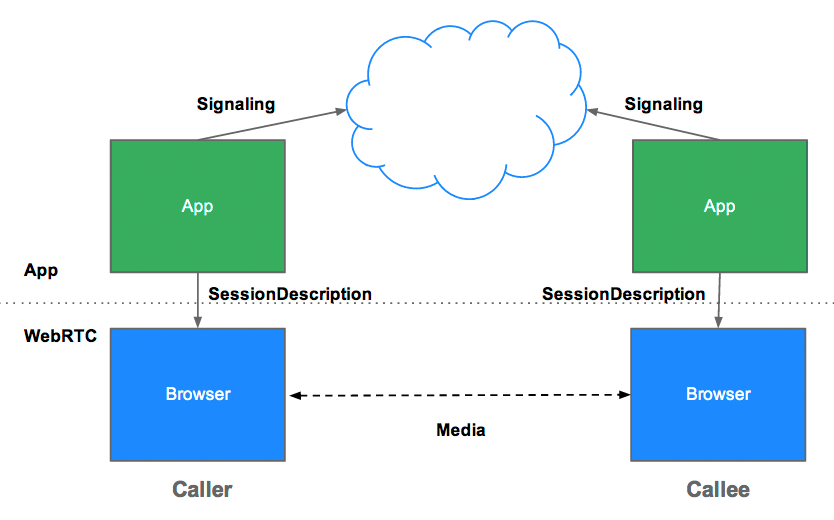
\includegraphics[scale=0.4]{jsep.png}
	\end{figure}
	
	WebSockets is a protocol implemented by browsers and servers to provide bi-directional communication between them\cite{WebSockets}. Once established, a session with a client communicating with the server is left open for the server to send messages to the client and vice versa, making it a good candidate for signalling with a WebRTC application which needs peers to be able to reliably send messages back and forth through the server. Over this WebSockets session, SIP messages will be sent. SIP is a communication protocol that does not specify how signals are transported but how these signals are defined. The transaction model defined by SIP is similar to HTTP with each SIP request being matched by a SIP response. An example of a SIP over WebSockets transaction:\cite{SIP Over WebSockets}
	
Initial handshake with WebSockets signalling server over HTTP \\
Alice -\textgreater\ proxy.example.com (TLS)
\begin{lstlisting}[tabsize=1,frame=single, basicstyle=\ttfamily\footnotesize]
GET / HTTP/1.1
Host: proxy.example.com
Upgrade: websocket
Connection: Upgrade
Sec-WebSocket-Key: dGhlIHNhbXBsZSBub25jZQ==
Origin: https://www.example.com
Sec-WebSocket-Protocol: sip
Sec-WebSocket-Version: 13
\end{lstlisting}
Switching to WebSockets protocol \\
proxy.example.com -\textgreater\ Alice (TLS)
\begin{lstlisting}[tabsize=1,frame=single, basicstyle=\ttfamily\footnotesize]
HTTP/1.1 101 Switching Protocols
Upgrade: websocket
Connection: Upgrade
Sec-WebSocket-Accept: s3pPLMBiTxaQ9kYGzzhZRbK+xOo=
Sec-WebSocket-Protocol: sip
\end{lstlisting}
SIP REGISTER request letting the server know of Alice's "location" \\
Alice -\textgreater\ proxy.example.com (TLS)
\begin{lstlisting}[tabsize=1,frame=single, basicstyle=\ttfamily\footnotesize]
REGISTER sip:proxy.example.com SIP/2.0
Via: SIP/2.0/WSS df7jal23ls0d.invalid;branch=z9hG4bKasudf
From: sip:alice@example.com;tag=65bnmj.34asd
To: sip:alice@example.com
Call-ID: aiuy7k9njasd
CSeq: 1 REGISTER
Max-Forwards: 70
Supported: path, outbound, gruu
Contact: <sip:alice@df7jal23ls0d.invalid;transport=ws>
;reg-id=1
;+sip.instance="<urn:uuid:f81-7dec-14a06cf1>"
\end{lstlisting}
OK response \\
proxy.example.com -\textgreater\ Alice (TLS)
\begin{lstlisting}[tabsize=1,frame=single, basicstyle=\ttfamily\footnotesize]
SIP/2.0 200 OK
Via: SIP/2.0/WSS df7jal23ls0d.invalid;branch=z9hG4bKasudf
From: sip:alice@example.com;tag=65bnmj.34asd
To: sip:alice@example.com;tag=12isjljn8
Call-ID: aiuy7k9njasd
CSeq: 1 REGISTER
Supported: outbound, gruu
Contact: <sip:alice@df7jal23ls0d.invalid;transport=ws>
;reg-id=1
;+sip.instance="<urn:uuid:f81-7dec-14a06cf1>"
;pub-gruu="sip:alice@example.com;gr=urn:uuid:f81-7dec-14a06cf1"
;temp-gruu="sip:87ash54=3dd.98a@example.com;gr"
;expires=3600
\end{lstlisting}

	Once two peers have registered, one of them can send an invite to another through the server in the form of an INVITE request to form a signalling channel between them which WebRTC uses to establish a peer connection and data channel. To create this peer connection, it uses interactive connectivity establishment (ICE) to find a list of the possible IP's and ports of each peer which are then sent through the server. Once this is done, the data channel can be formed and packets can be sent peer-to-peer. These packets are managed and secured by Secure Real Time Transport Protocol (SCTP) for media and Stream Control Transmission Protocol(SCTP) for non-media and encrypted by Datagram Transport Layer Security (DTLS) \cite{WebRTC Data Channel Establishment Protocol}.
				
\chapter{Specification}
	\section{Deliverables}
	The first intermediate product will be the signalling server written in Java. This will handle the exchange of client meta data in order to establish the connection between two peers using the web application. I plan to overlap the development of this with the development of the data transfer functionality and user interface of my second deliverable, the web application as manually testing the signalling server will be a lot easier with a partially developed application to test it with.
	
	The first end deliverable will be the client side web application the user interacts with in order to select a file as well as handling sending the meta data to the signalling server and managing the peer-to-peer data transfer and media streaming. This is broken down into several intermediate products, the data transfer functionality, the media streaming functionality, the peer-to-peer network and the user interface. I plan to produce the data transfer functionality first along side the user interface to allow for manual testing. After I have implemented data transfer, I will work on media streaming and forming the peer-to-peer network topology. 
	
	The second end deliverable will be the final report containing documentation and analysis using the metrics from my application, comparing how it and technologies behind it perform in comparison to others, focusing in particular on how peer-to-peer over the browser (WebRTC) compares to other methods of data transfer and media streaming.
	
	\newpage
	\begin{figure}[h!]
		\caption{Schedule of Activities}
		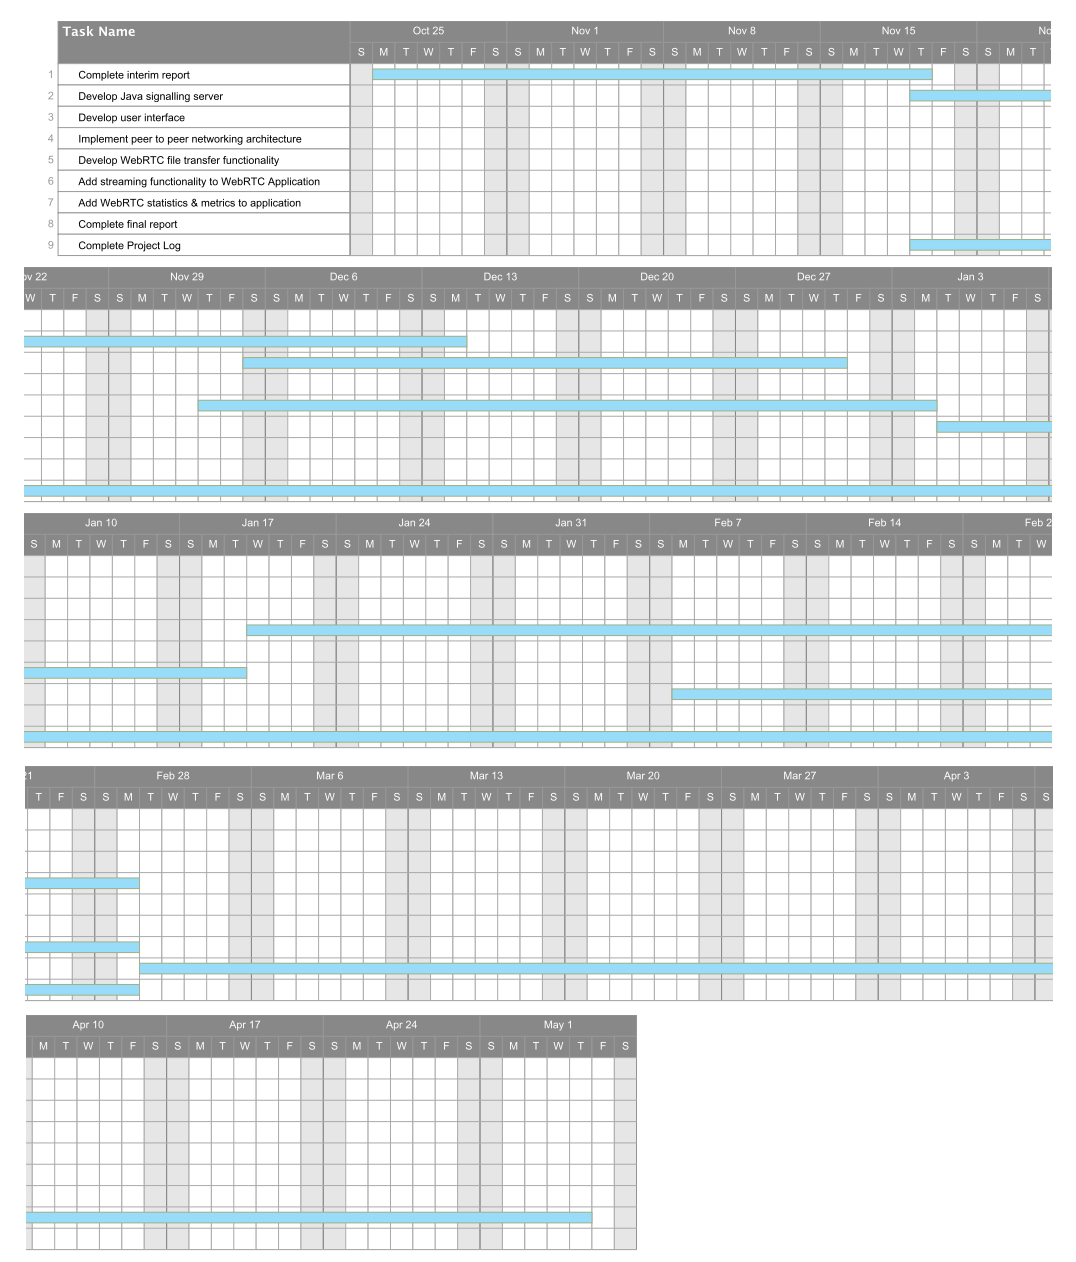
\includegraphics[scale=0.5]{ganttchart.png}
	\end{figure}
	\newpage	
	
\section{Risk Analysis}
	\scalebox{0.6}{
		\begin{tabular}{@{}|l|l|l|l|l|@{}}
			\toprule
			\textbf{Risk}                                      & \textbf{Probability (1-5)} & \textbf{Impact (1-5)} & \textbf{Mitigation}                                                                                                  & \textbf{Contingency}                                                                            \\ \midrule
			Illness/Injury                                     & 4                          & 3                     & \begin{tabular}[c]{@{}l@{}}Reserve time for illness\\ Be hygienic\\ Eat healthy\\ Exercise\end{tabular}              & \begin{tabular}[c]{@{}l@{}}Allow time for recovery\\ Take medicine to aid recovery\end{tabular} \\ \midrule
			Inaccurate estimations                             & 3                          & 3                     & \begin{tabular}[c]{@{}l@{}}Be liberal with estimations\\ Reserve time for deliverables behind schedule\end{tabular}  & Adjust scope of project                                                                         \\ \midrule
			Data loss                                          & 1                          & 5                     & \begin{tabular}[c]{@{}l@{}}Use a version control system\\ Keep local backups\end{tabular}                            & Recover data from Git                                                                           \\ \midrule
			Uncommunicative stakeholder                        & 1                          & 3                     & Ensure regular meetings with stakeholder                                                                             &                                                                                                 \\ \midrule
			Stakeholder turnover                               & 1                          & 4                     & N/A (out of my control)                                                                                              & Get new stakeholders                                                                            \\ \midrule
			Project scope too large                            & 3                          & 4                     & \begin{tabular}[c]{@{}l@{}}Research enough to be certain in project scope\\ Be liberal with estimations\end{tabular} & Adjust scope of project                                                                         \\ \midrule
			Technologies too immature/insufficient for project & 2                          & 4                     & Research technologies beforehand                                                                                     & \begin{tabular}[c]{@{}l@{}}Find alternative technologies\\ Adjust scope of project\end{tabular} \\ \bottomrule
		\end{tabular}
	}

	\section{Quality Analysis}
	The main measure of success will be the web application's performance in it's ability to transfer \& stream data between two peers. To track this, I will implement metrics using the WebRTC "getStats" statistics API, which allows for monitoring of the bandwidth usage, packets lost and network delay within a data channel between two peers. I will then gather these statistics in two different cases, one where there is no formal network structure (to find a baseline) and then when the many-to-many network has been implemented to compare if the structured peer-to-peer network does improve performance of the application. This network will also have it's own monitoring to ensure that peers are being correctly organised. Further to this, I will also compare the speeds of file transfer with other services such as DropBox through their API, however this may prove unrealistic as these services will be running on more powerful servers. To certify that the user-experience is acceptable, the application will also be user-tested. The signalling server will be load tested in isolation to make certain it can handle multiple requests to ensure it does not bottleneck the application. 
			
	\chapter{Methodology}
	I chose to use an alternative methodology to the waterfall model because it lacks the ability to adapt to changes in a project deadline. Due to the way waterfall is structured into different phases that must be completed sequentially, often when changes such as new requirements occur, all these phases must be repeated in order to account for this. Iterative methodologies take an approach that can adapt to these changing requirements because they utilise short development cycles and focus on developing small modules of a product at one time, making it easier to revise a product if necessary. This is particular useful in my project as it is relatively experimental and the requirements of it may change regularly. 
		
	Thus, as a way of tracking the progression of my project, I plan to use an iterative and evolutionary methodology. This is used within software development as a way of incrementally developing applications through small cycles. Whilst it will be similar to scrum, it will not have the stricter framework surrounding it that requires a product owner and scrum master. This methodology will be relatively simple and based around a backlog of tasks from which a developer pulls from in a limited amount, normally 1 or 2 tasks at a time which will are then pushed through the development work flow.
		
	In my case, the work flow will be relatively simple:
	\begin{enumerate}
		\item To Do
		\item In Progress
		\item Code Review
		\item Manual Testing
		\item Done
	\end{enumerate}
		
	During the "In Progress" step of the work flow, I will use a test driven development (TDD) process in which tests are written first and then code is wrote to make the test work. However, I will be fairly lenient with this, only using this process on parts of the code that require stringent testing as writing unnecessary tests will take up development time. 
	\begin{figure}[H]
		\caption{
			Test-Driven Development (TDD) Cycle
			\cite{TDD Diagram}
		}
		\centering
		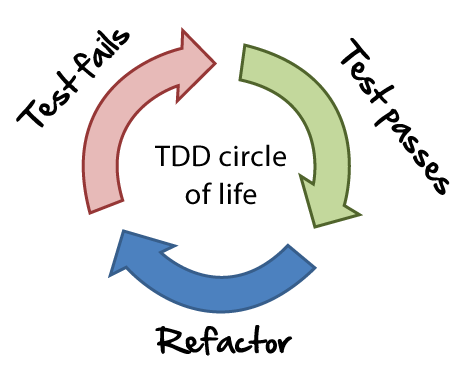
\includegraphics[scale=0.5]{tdd-circle-of-life.png}
	\end{figure}
	During the "Code Review" step, I plan to self-evaluate the task I have completed. On top of this, I will run static code analysis tools (such as FindBugs/PMD for Java) if the task is a coding task and use the code review section StackExchange to get second opinions. If it passes the code review step and it is possible to do so, I will black-box test the task from a user's perspective to see that it actually works as intended. Once every task forming a feature is completed, I will manually test the feature as a whole to see that each task has integrated together as planned.
	
	To visualise this workflow, I will use the open source web application "Kanboard" which I have hosted on an Amazon Web Instances EC2 Instance. This will allow me to keep track of progress throughout the duration of the project. To manage the actual changes made to the project files, I have utilised the version control system Git with a private GitHub repository containing my project.
	
	\chapter{Prototyping}
		\section{Architecture}
			\begin{figure}[H]
				\caption{Application Architecture}
				\centering
				\includegraphics[scale=0.5]{application-architecture.png}
			\end{figure}
			To organise the client-side application, I coded each layer of JavaScript in individual modules, separated by their responsibilities. These layers consisted of the presentation code that had the responsibility of listening to and manipulating the document object model, the peer-to-peer network code that worked with WebRTC to established the peer connections and the signalling code that established the socket connection. By separating these layers into their own modules, the application was left with a relatively simple architecture which can be easily extended and maintained without causing side-effects in other unrelated modules.
			
			In order to model these modules and to manage dependencies between them, a build tool called Browserify was used. Traditionally, all of the JavaScript files are added using script tags within the html document they are assocaited with. Instead, this tool allows you to add a JavaScript file as a dependency within another by using a function "require('module')" to simulate the modular structure Node.js uses. This makes it clear which dependencies each modules require. To do this, The JavaScript files are wrapped in a global function which Browserify can then export and bundle together into one larger JavaScript file using a command line interface which is then referred to in the HTML document. By doing this, the client side JavaScript can also access node modules that you may have installed within the project as well.
			
			The server uses the Express.js web framework for two purposes, to serve files to the browser by resolving URLs to static resources and to also provide the RESTful API which the client-side JavaScript communicates with by routing HTTP requests to functions in server.js. As the server-side functionality was minimal, there was no need for more than one JavaScript module to separate the functionality. Although in the future, if the web server functionality such as the API is expanded, it may need to be moved to it's own module. Both the server and the client also uses the Socket.io library to support bi-directional communications between server and client via the WebSocket Protocol. 
			
			\subsection{Application Flow}
			\begin{figure}[H]
				\caption{Application Flow}
				\centering
				\includegraphics[scale=0.6]{application-flow.png}
			\end{figure}
			
		\section{Signalling}
			\subsection{1st Iteration - Spring Boot}
				\subsubsection*{Spring WebSockets Over STOMP}
				The first prototype of the signalling server for Transfer4me was implemented using spring boot. This is a part of the Spring application framework emphasising convention-over-configuration, making it faster and easier to produce a working prototype. To support the WebSocket protocol, Spring uses the "STOMP" sub-protocol to model the message sent between server and client, STOMP is very similar to HTTP in how it models the message but is sent over TCP once the socket is established. Using the STOMP JavaScript client, an application can subscribe to several destinations and listen for events (by asynchronous callbacks) or publish events using a send method that takes a string identifying the event (which in this case is "signal") and another string representing the message. The architecture that was created on top of this protocols used rooms that were created when a user uploads a file designated via a URL which the recipients then subscribe to when they load the page.

				To create the room that the users reside in, the client that uploads the file fires a request to the server using an endpoint independent of WebSockets. When the server receives this request, it generates a Room object and a random unique integer that serves as its identifier. This room is then added to a list of rooms and the Id is returned to the client in the response. The uploader then uses this id to subscribe to the room over WebSockets. When this connection is established, the server creates a user object and adds it to the correct room. This ID is then appended to the base URL of the page for the uploader to share. The recipient then loads the URL but only joins the room at the point at which it is necessary (when the recipient either chooses the download or stream button), This is a tactic called "Lazy initialization" and by using it, the server only has to cope with the load from the sockets that actually need to be connected as opposed to users that may be idly sitting on the page.
							
				\subsubsection*{Problems}
				The main problem I found with the Spring implementation was in its limited functionality. It was extremely hard to implement sending messages to individual specific sockets which limited how multiple peer connections could communicate within the same room as they would all be receiving every signal being exchanged. This could be avoided by making each client application only use the messages that were destined for it by appending an identifier to each message but that would not stop the clients from receiving the messages, only how they used them. As a result, this is not a viable solution as it leaves the application open to man in the middle attacks as a user could easily modify the client-side application to log all of the messages that it received which is a major issue in this case where the the majority of the messages sent will be WebRTC meta data containing information such as your IP address.
				
			\subsection{2nd Iteration - Node JS}
				\subsubsection*{Socket.IO}
				To solve the problems found with the Spring implementation, the server was refactored using Node.js as a replacement. This is a server-side environment that uses modules written in JavaScript to produce web applications. In my case, choosing this environment gives me the benefit of developing the full stack in one language, making the process a lot easier. Node.js maintains support for WebSockets through the Socket.IO library which offers extended functionality over the Spring counterpart. Socket.IO models communication using the concepts of "rooms" and "namespaces" where a namespace is represented by the endpoint a socket connects to and rooms are channels within this that users can be a part of, allowing for communications to be separated. By default, every socket that connects to a namespace has it's own room which means Socket.IO can broadcast events to specific user's rooms solving the security issues that I was unable to with the spring implementation. As a result of this, the architecture of the server was slightly changed to reflect this new functionality as there was no longer a need to have an object to specifically represent a user. 
				
				\begin{figure}[H]
					\caption{Signalling establishment sequence}
					\centering
					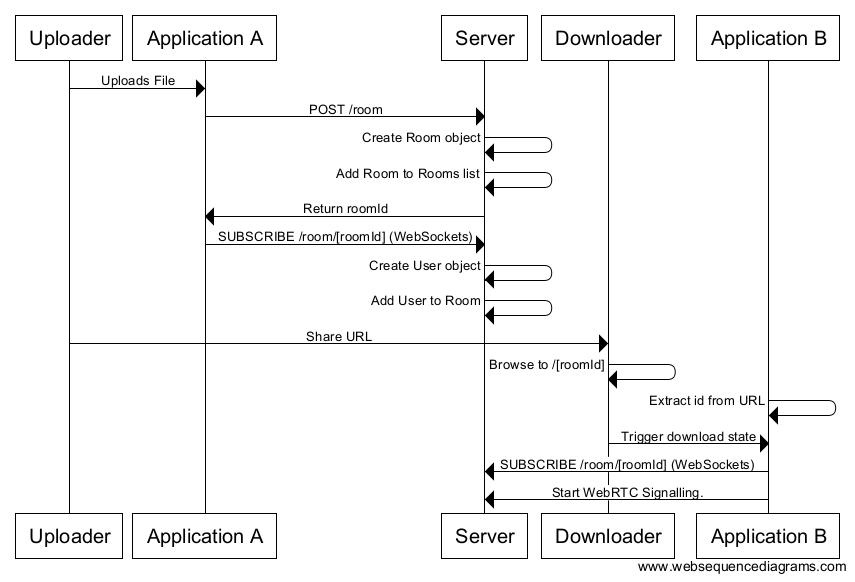
\includegraphics[scale=0.5]{signalling-establishment-sequence.png}
				\end{figure}
				
				\subsubsection*{API}
				At this point, the API was extended order to support the changes in the client side web application's interface. Another endpoint was added to retrieve the file type of the file uploaded as the application would let you select the stream option for any file (including files such as a text document) which would evidentially cause it to break. By adding this endpoint, it meant that the client-side application could find out the file type and only present you with the corresponding options for this file type. It was also extended to provide basic authentication by modifying the current new room endpoint to generate a password if specified and adding a new endpoint to validate the password. 
				
				As these endpoints were added, I realised that the API was becoming inconsistent and should be restructured for clarity. As a result, they were re-factored using a RESTful approach. REST (Representational State Transfer) is an architectural style specifying that an endpoint into a system (such as a URI) should be built around resources with methods for retrieving and manipulating this resource. In the real world, these methods generally translate into HTTP verbs such as GET and POST. For example to add a room, a POST request is sent to the URI "/room" and to retrieve a room, a GET request is sent to "/room/{roomId}". These guidelines allow for an easily maintainable API as well as providing the client web application with a predictable and consistent group of URIs to code against. As a RESTful API is modelled in terms of resources, it does not hold the state of a client's journey throughout the web application and thus, this is left up to the client consuming the resource which in this case is a JavaScript application. By doing so, it means the server is under less load and is in a better state to be scaled.
				
				\begin{description}
					\item [API Documentation]
				
					\item[GET /room] 
					Adds a unique room to the list of rooms on the server. Returns a JSON object containing a UUID for the room and, if the passworded field is present in the request body, a random string password.
						
					\item[GET /room/\{roomId\}/fileType] 
					Returns the MIME type of the file associated with the room.
					
					\item[POST /room/\{roomId\}/password] 
					Takes a password from the request body and compares it with the password associated with the room. If the password is correct, it will add a cookie containing the password to the response. If the password is false, it will return a 401 Unauthorized HTTP status code.
					
				\end{description}
				
				\subsubsection{JSON}
				Both the socket implementation and the API transfer data in a format known as JSON (or JavaScript Object Notation) in order to remain consistent throughout the application. This was chosen as the data transfer language because JavaScript has native functions for parsing to and from JSON as opposed to other common alternatives such as XML, I also found that JSON is a lot easier to read as a human than XML and the benefits of XML such as custom schema support was not deemed necessary.
		
		\section{Peer to Peer Communication}
			\subsection{One-to-one peer connection}
			As a starting point, I worked on using WebRTC to establish a simple peer connection between two clients. This process is done through negotiation using offers and answers representing what each client wants from the other client and what the client is willing to offer such as media streams and constraints on these. These parameters are modelled using a protocol called "Session Description Protocol" or "SDP" and is generated by WebRTC. In a traditional WebRTC architecture, the peer that sends the offer tends to have something to offer (such as a stream). The architecture for transfer4me is slightly different in this sense as the offer is sent from the recipient peer even though the uploader is the peer with something to offer. This arises from how transfer4me uses WebRTC as a means to transfer files as opposed to its conventional purpose of establishing real-time communications. Due to this, the negotiation process is closer to reflecting the "request-response" pattern used in HTTP transactions more than it does an "offer-answer" model. This architecture also improves performance as the uploader does not have to send and maintain offers to every peer that joins the room which would introduce a large amount of unnecessary load especially if the recipient peer joins but never downloads or streams the file. Instead, the offer is "lazily initialized" by the recipient peer in the sense it is only created and sent at the point it is needed which in this case is when they either opt to download or stream the file, this way the uploader only deals with the recipients that request the file. 
			
			Once the offer SDP is created, it is stored as the local description and sent to the uploader via the signalling channel. The uploader receives this, sets it as the remote description and creates an answer SDP which is again set as their local description and sent back to the recipient via the signalling channel. Both these SDPs contain "ICE candidates" which detail potential IP addresses that can potentially be used to establish a connection. However, how WebRTC handles the the retrieval of these ICE candidates depends on the browser. Chrome supports a concept called "trickle ICE" where ICE candidates can be sent on-the-fly as they are received regardless of whether the sdp has been sent or not whereas Firefox is limited as it does not support this and all candidates have to be sent with the sdp. 
			
			\begin{figure}[H]
				\caption{Peer Connection Establishment Sequence in Chrome}
				\centering
				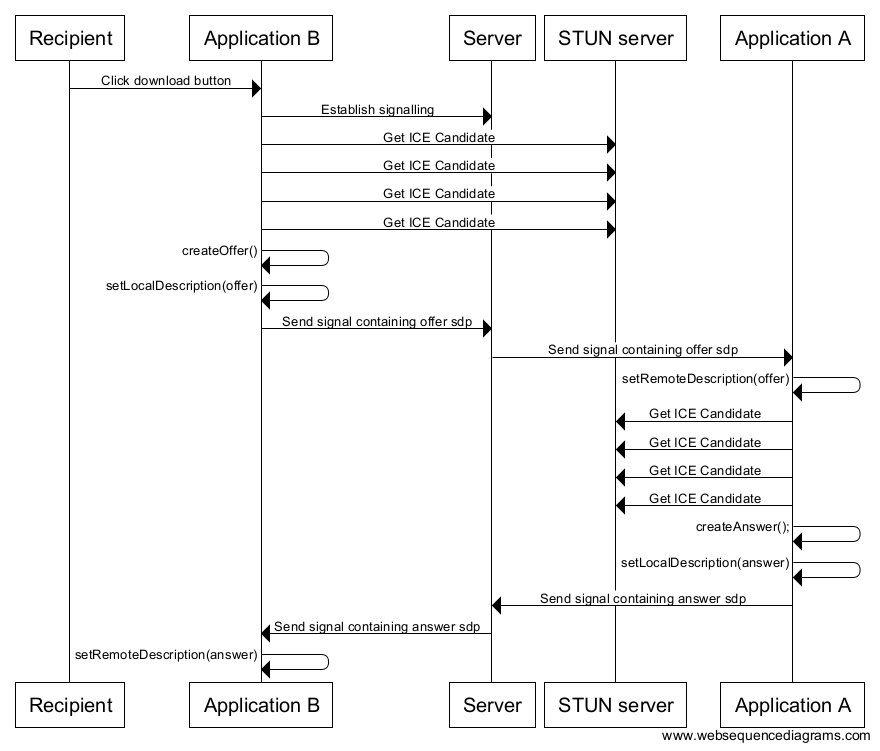
\includegraphics[scale=0.5]{peer-connection-establishment-sequence-chrome.png}
			\end{figure}
			
			\begin{figure}[H]
				\caption{Peer Connection Establishment Sequence in Firefox}
				\centering
				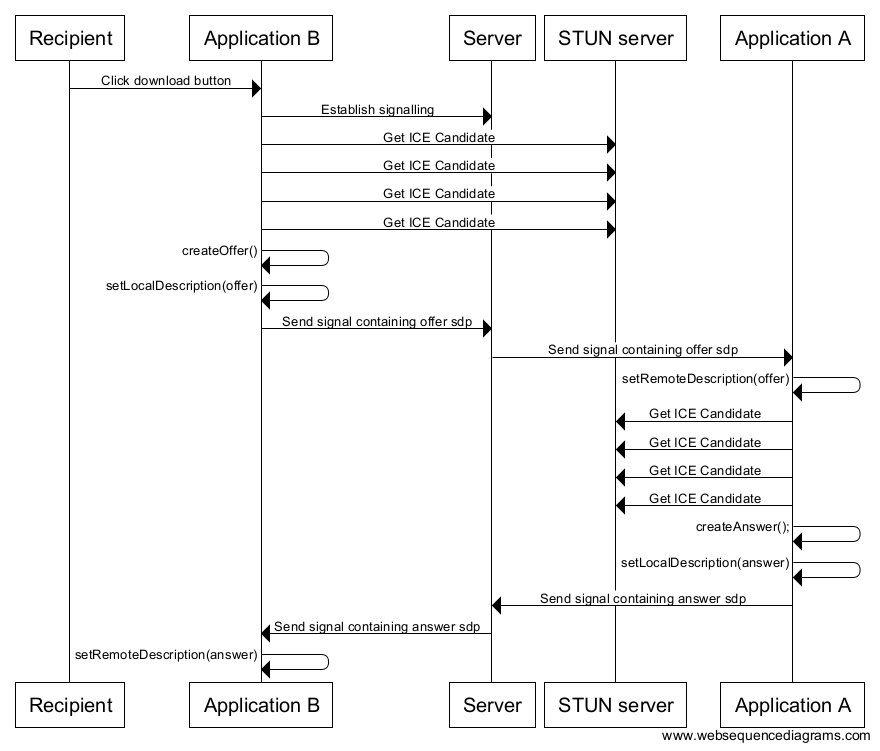
\includegraphics[scale=0.5]{peer-connection-establishment-sequence-firefox.png}
			\end{figure}
			
			\subsection{Using RTCDataChannel to transfer files}
			In order to download a file, the recipient creates a new DataChannel using the RTCPeerConnection API which is added to the offer to be sent to the uploader. Once the connection is established, the uploader waits for the addition and establishment of this RTCDataChannel via an asynchronous event listener. After this, how the file is sent depends on the browser. In Firefox, once the DataChannel reaches it's open state, a callback is fired which sends the file through. On the recipient peer's client, an event listener waits for messages to be sent through which then catches the file and saves it to the disk. However, Chrome's implementation of RTCDataChannel has a size limit on the messages that can be sent meaning the file has to be sliced into several smaller parts which can then by reassembled by the recipient (a process called chunking). The major problem with this approach is that it significantly bottlenecks how fast a file can be sent to the recipient in Chrome. Although this allows for cross-browser file sharing, sending files from Firefox to Firefox will always be faster for downloading files via the application. Once this file has been received, it is then saved to disk by reading the file in as a data URI and then appending an element to the html with this URL as the reference. A mouse event is then used to simulate the click of this element which triggers the file to download. 
			
			\begin{figure}[H]
				\caption{File sending sequence in Chrome}
				\centering
				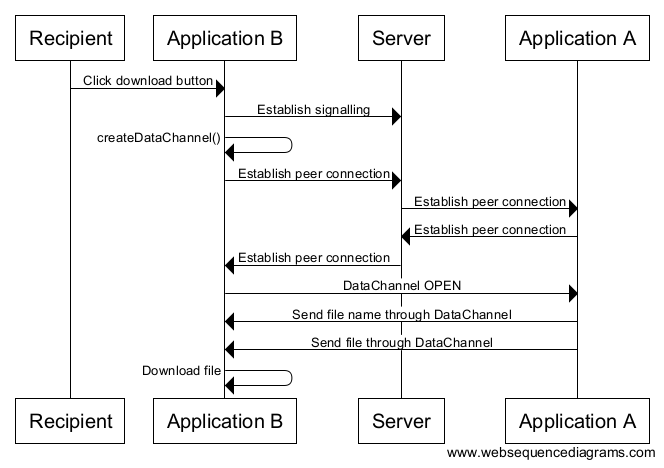
\includegraphics[scale=0.5]{file-sending-sequence-chrome.png}
			\end{figure}
			
			\begin{figure}[H]
				\caption{File sending sequence in Firefox}
				\centering
				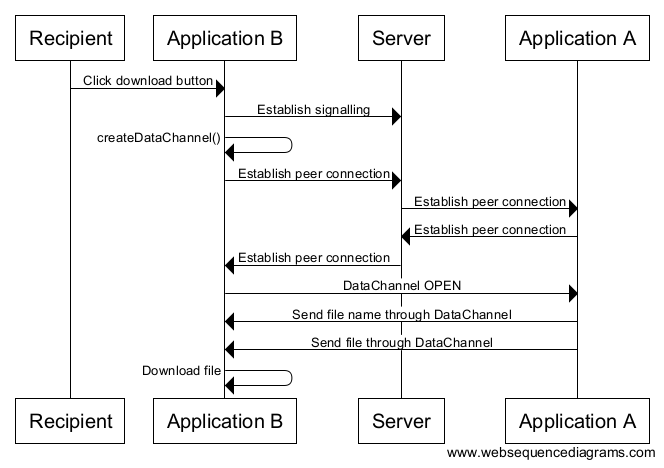
\includegraphics[scale=0.5]{file-sending-sequence-firefox.png}
			\end{figure}	
			
			\subsection{Streaming media via peer connection}
				\subsubsection{Audio}
				In order to stream Audio via WebRTC, a media stream is added to the peer connection by the uploader once the offer has been received from the file recipient. Once the answer sdp containing the media parameters for this stream has been sent back and the peer connection is established, an event listener on the recipient application listens for the event signalling the addition of this stream and uses the HTML5 Audio API to create a new audio tag which is appended to the html. The source attribute of this tag is set to the incoming stream and the audio player is set to play automatically. It is important to note that the stream actually starts to play when it is created by the uploader as it is a "live stream" and if there is any latency issues between the two clients or if the recipient decides to pause the player, the stream will carry on and they will miss parts of it.
				
				To avoid the problems with live streaming, the recipient could instead completely download the file from the uploader using RTCDataChannel and then play it using the HTMl5 audio element. By doing so, they would be able to pause and control it. However, the problem with this is that it puts a limit on the size of the file that can the uploader can stream to a recipient as the RTCDataChannel has a size limit on what can be sent through.

				\subsubsection{Video}
				I originally planned on also adding video streaming to the application. However, when I looked into this, the part of the MediaStream processing API drafted by W3C that would capture video as a stream has yet to be implemented by any browsers. Similar to how audio is captured, The captureStreamUntilEnded() function would return a MediaStream containing both the audio and video tracks of a file which could then be passed to the peer connection and played by a HTML5 video element on the recipient's application.
				
				These issues could also potentially be avoided by downloading the file via RTCDataChannel before playing it with a HTML5 video element as it means the uploader would not have to convert the file to a media stream in order to transfer it to the recipient.
			
			\subsection{One-to-many peer connections}
			Switching to the Node.js implementation of the server allowed me to implement one-to-many peer connections with ease. To do this, the uploader instantiates new peer connections and adds them to an array which are then used to communicate with the recipients which only has to hold one peer connection. Each message sent via the signalling server contains the socketID of the user it is from and the user it is destined towards, which is then extracted by the server and used to send messages to only them, this way no socket information can be exposed to anyone except for the user it belongs to. One of the big disadvantages of this is the potential amount of load on the uploader as they now have to maintain and search through an array of peer connections and as this gets larger, the larger the load. To manage this, the recipient sends a message to the uploader signifying to close the connection and remove it from the array as soon as the recipient has downloaded the file. In the future, I also hope to add this functionality for when a MediaStream ends but currently the MediaStream API in Firefox has no way of establishing when a stream has finished.
			 
			\begin{figure}[H]
				\caption{one-to-many peer connections}
				\centering
				\includegraphics[scale=0.5]{One-to-many.png}
			\end{figure}	
						
			The better way to avoid overloading the uploader would be through maintaining a pool of nodes that have already downloaded the file (or seeds) on the signalling server from which incoming peers can download the file from with each of these seeds maintaining an array of peer connections. This way, a limit can be set in order to prevent one seed from becoming burdened with too many recipients. Once each seed has reached its limit, it would alert the signalling server and other incoming peers would be redirected to download or stream from another seed. Once these incoming peers download the file, the peer connection between them and the seed is disconnected and they become seeds themself, forming a new network of peers. When every seed in the pool is saturated with a peer, the rest can then be enqueued to a FIFO queue and wait for a seed to become free. This approach would ensure that the file could propagate to new incoming peers even when the the original uploader has disconnected from the room as long as there was always one seed. One constraint with implementing this in my application is that only the downloaders could be considered valid seeds as they are sent the actual file whereas streamers would only be sent an audio stream of that file.
			
			\begin{figure}[H]
				\caption{many-to-many peer connections}
				\centering
				\includegraphics[scale=0.5]{many-to-many.png}
			\end{figure}	
			
			One of the limitations of my approach in developing the application was that I geared the development towards achieving one-to-many peer connections without thinking about the long term goal of many-to-many connections, making the introduction of this functionality a difficult task as it will take a significant amount of code re-factoring.
			
			\subsection{Data Aggregation}
				\subsubsection{Data Collection}
				In order to gather statistics on the peer to peer connections within a room, I created two new functions, one for streaming and one for downloading, that are called on the recipients application in order to collect information about the transfer of data. For the streaming data, I created a function that utilised the WebRTC GetStats API which returns a raw data object containing information about the connection including the streams and data channels that exist within it. The function sets up the getStats function and then extracts data from the resulting data object in a callback, the data is then sent  to the signalling server along with the room id and the socket ids representing the user at each end of the connection. In the download data gathering function, I was unable to use the getStats API as it does not contain useful statistics about the DataChannel, instead I created a custom object that contains the amount of bytes that was sent through to the recipient in each chunk. In both functions, this data is sent to the signalling server which then adds file meta-data to the statistics object such as size and type which is gathered when the file is initially uploaded. This information is logged to a file using a logging library called Winston that formats it with a time stamp. Winston is built to provide a simple interface to log to and query from multiple locations (or "transports") which would allow me to easily scale my application in the future.
				
				\subsubsection{Data Visualisation}
				To monitor the application, I thought it would be a good idea to model the data I was receiving from the recipient using a data visualisation tool. There are a number of tools and libraries that enable developers to do this such as D3.js \& Charts.js. Initially, I chose to use a pre-built data visualisation server built with node.js called Lightning-vis which uses a REST API to communicate with. This way, I was able to live stream the data sent to the signalling server to the data visualisation server and watch the connections in each room in near real-time. Instead of directly interfacing with the REST API, I chose to use a JavaScript API client library that obfuscates the API and makes it easier to code against. Using this, I was able to create a lightning server session for each room created on my application and post the data to visualisations contained within them. However, as I was developing with the server and API client, I found it didn't have the functionality I was looking for. For example, once I created a visualisation in a session, I wasn't able to add more data series, only update the ones that previously existed, this meant that I wouldn't be able to add series to represent recipients as they joined and left the room. Another issue was that I found that the JavaScript API client was still quite buggy and I had to go into the code to fix it. Overall, I felt it would be better to approach data visualisation with a different library instead of expending any more time trying to make it work. However, if these problems were fixed in the future, this server would have been extremely beneficial as it I could use it to find bottlenecks in the code.
				
				\begin{figure}[H]
					\caption{Lightning Viz Session}
					\centering
					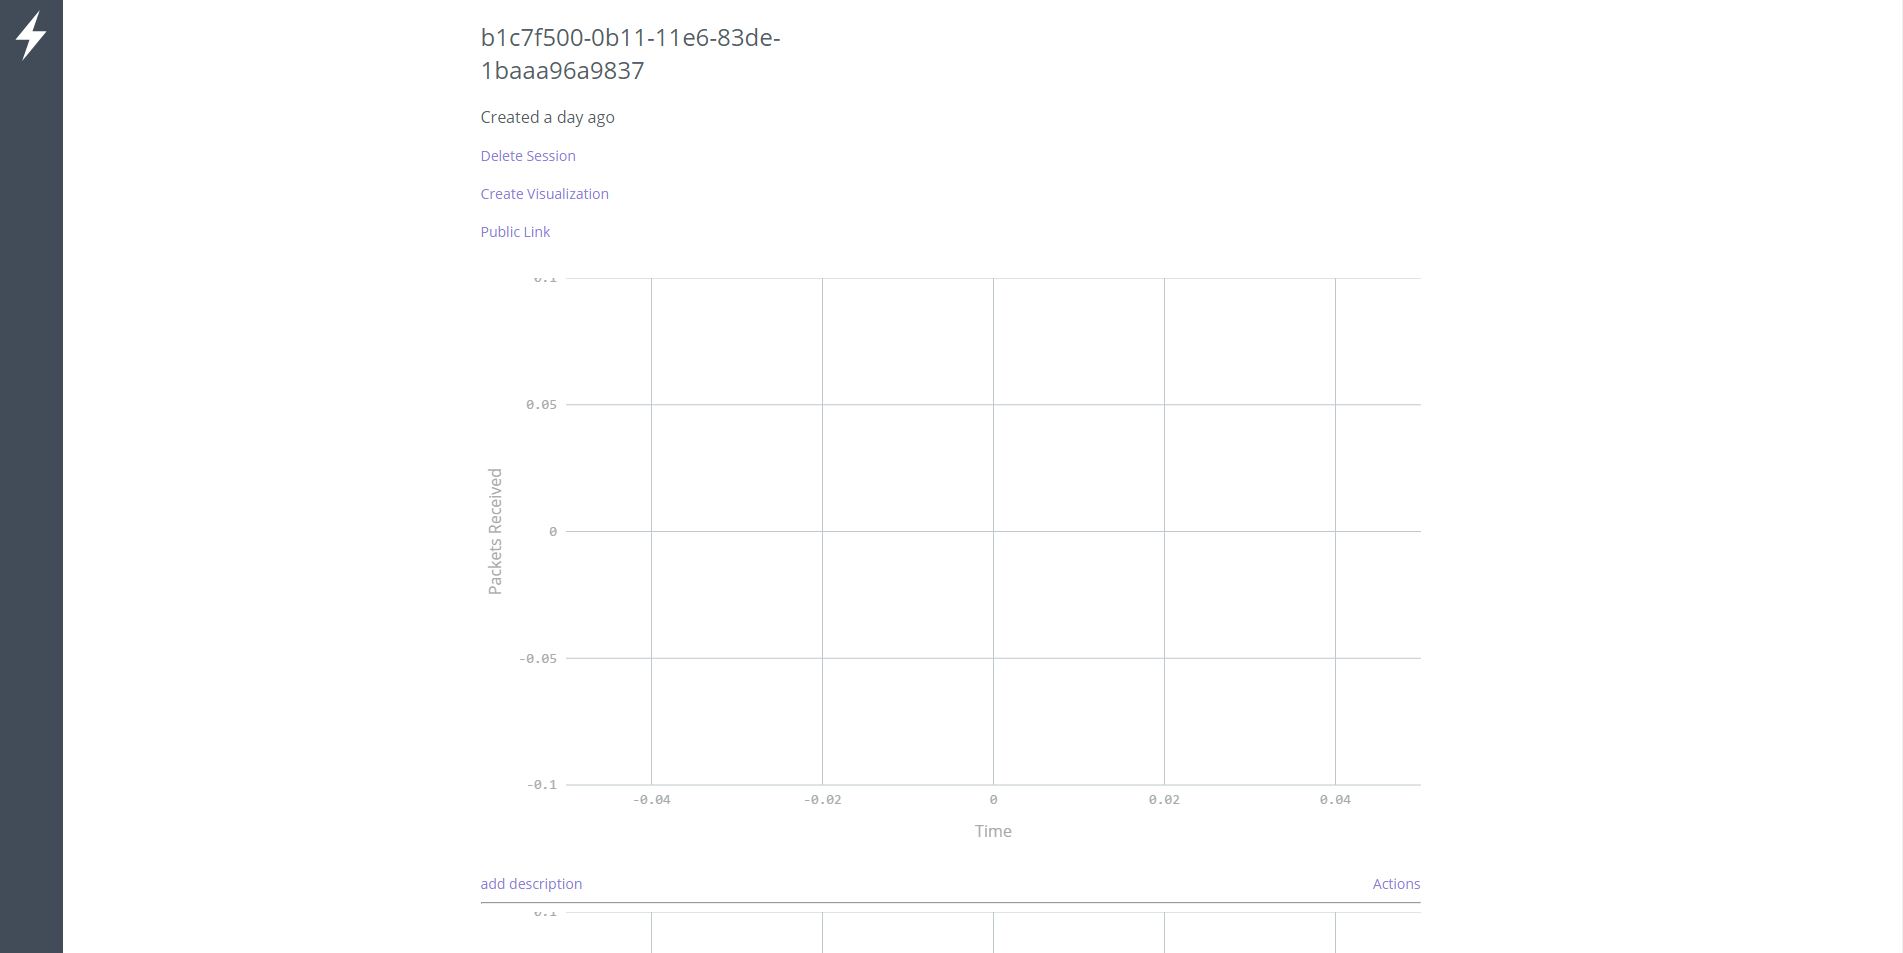
\includegraphics[scale=0.25]{lightning-viz.png}
				\end{figure}	
				
				As an alternative, I found a lightweight JavaScript library called smoothie.js that used the HTML5 canvas element to produce live streaming graphs. I used this library to add graphs to the uploader's application, enabling them to see how fast th users connected to them are either downloading or streaming the uploaded file. To do so, I updated the statistics sent to the signalling server by adding a new field that contains how many bytes the recipient receives per second and then made the signalling server forward these statistics on to the uploader. Using smoothie.js avoided the problem I was having with the lightning-viz server as I was now able to add a series per recipient to the chart. However, one of the downsides of this is that now the data visualisation and processing is all handled within the application which presents two problems. First of all, it puts extra load on the application instead of passing it to a service built for this purpose (like lightning-viz) which is probably considerably more efficient at it and secondly by doing so, it means that only the uploader can view the visualised statistics for the room. Due to this, I feel like this solution should only be temporary and refactored at a later point.
				
				\begin{figure}[H]
					\caption{Smoothie.js Chart}
					\centering
					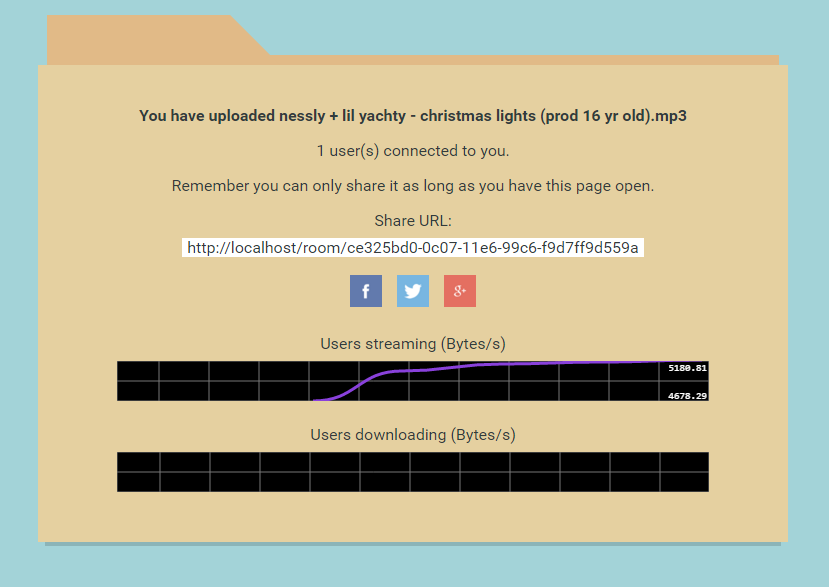
\includegraphics[scale=0.5]{smoothie-js.png}
				\end{figure}
				
		\section{Design}			
			As design and usability wasn't a key part of my project, I wanted to keep the design and structure of the web application simple and clean in order to minimise time and effort spent on it and to emphasise the sole purpose of the project. However, that said I feel the design of the application was still something that I needed to dedicate some time too as having a poorly designed site limited how easily I could test the application especially with the lack of unit tests. As you can see from figure 5.10, I went through multiple iterations to get to the final design which I felt fulfilled the goals of both making it easy to test and looking good.
	
			\begin{figure}[H]
				\caption{Iterations of Design}
				\centering
				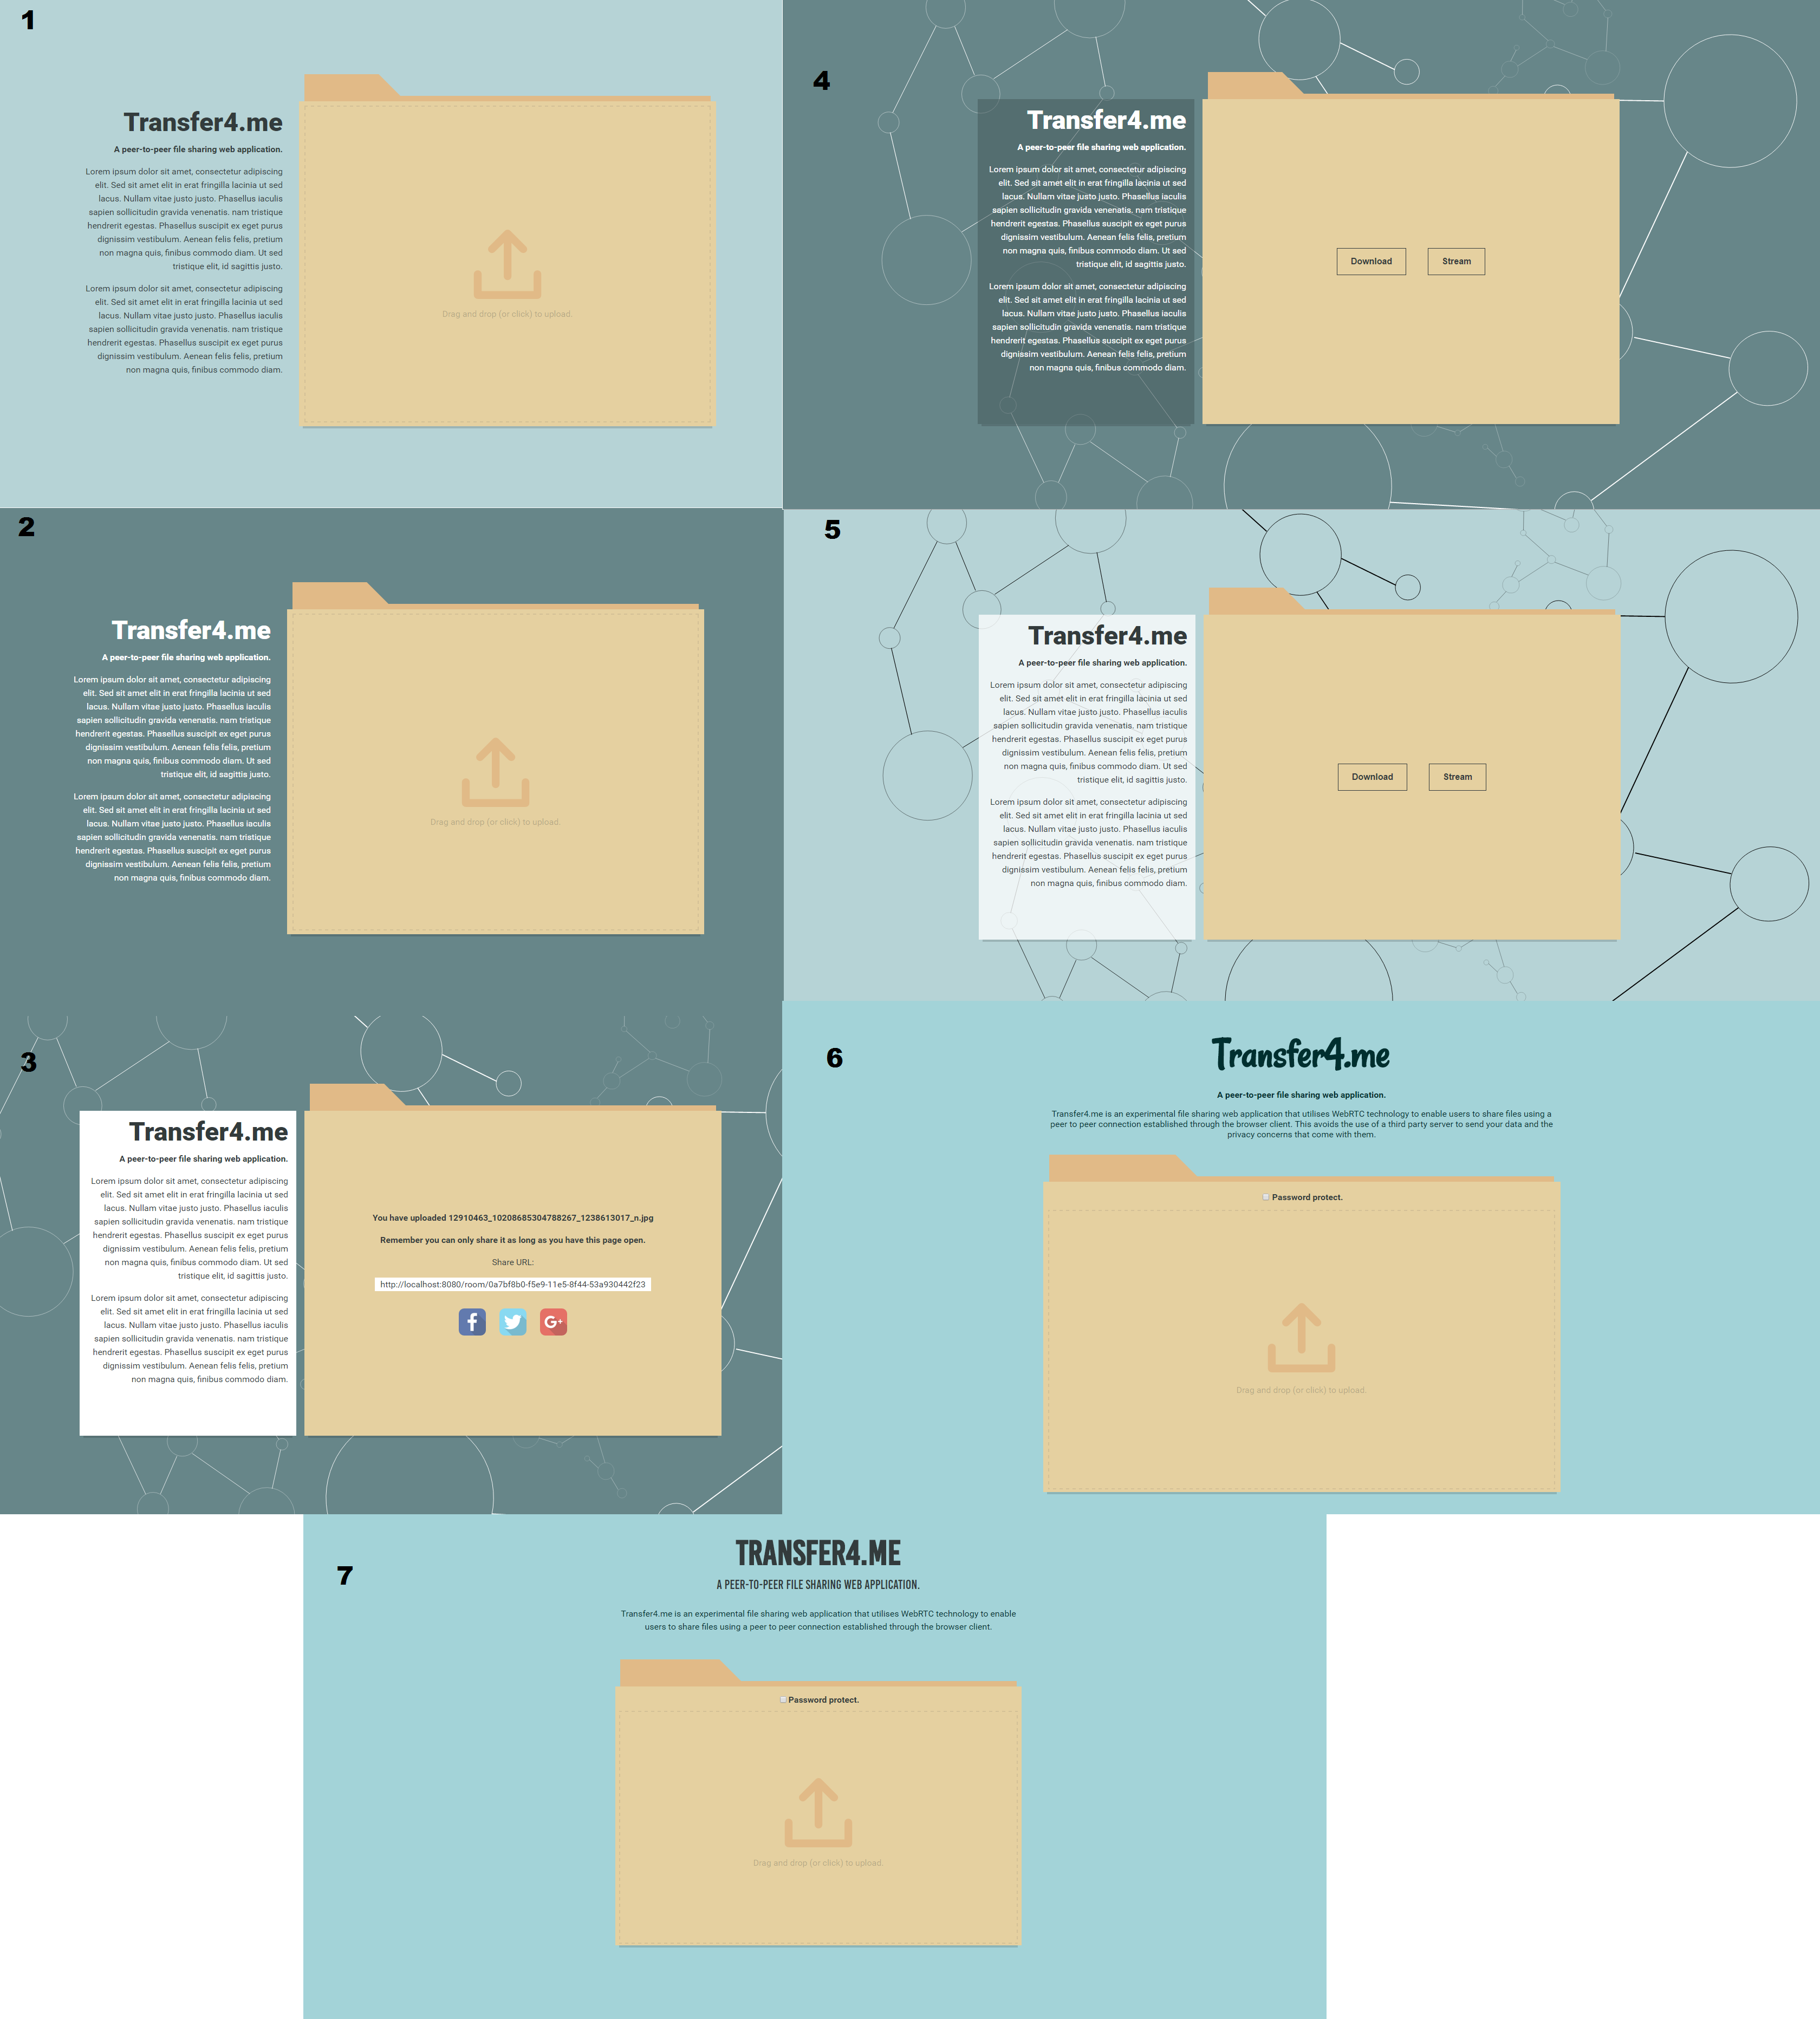
\includegraphics[scale=0.15]{design.png}
			\end{figure}
		
		\section{Technologies}
			\subsection{JavaScript Build Tools}
			In order to streamline the process of developing with JavaScript I used a tool called Browserify. As explained earlier, Browserify is a dependency management tool that allows you to use node.js modules in the browser as well as allowing you to modularize JavaScript to produce a more structured application. However, to compile the bundle of dependencies together, a command line interface is used. This can be done manually but starts to become inefficient when code is being changed constantly. An alternative to doing it manually is to automate the process using a task runner such as Gulp. Gulp is essentially a task runner that allows developers run all of the pre-processing needed to build their compile static resources. In order to automate the Browserify process, I found a gulp task that uses a JavaScript library called watchify that monitors JavaScript for changes and recompiles the bundle when it does. I was then able to run this gulp task through the command line whenever I was developing so that I did not constantly have to run Browserify myself. In the future, I could also use gulp for other tasks, for example if I refactored the application's css to use sass instead, I could create a task that watches the sass files for changes and automatically compile them.
			
			\subsection{Development Environments}
			I used WebStorm, an integrated development environment for JavaScript. I chose it because of the massive range of functionality I could utilise as opposed to basic text editors such as sublime. An example of this functionality was that I was easily able to run and specifically debug processes such as the browserify gulp task and the node.js signalling server through it which saved me a lot of time that I would have spent setting up a third party node.js debugger. It also allowed me to spot syntactic and semantic errors as I was writing the code and do things such as refactor names of functions without crawling through the rest of the code to see where it is used.
			
			\subsection{Git}
			Throughout the development process, I regularly committed code to my GitHub repository using the git command-line interface. This was a great habit to get into as it allowed me to track and log my work throughout as well as prevent any risk of accidental data loss or overwrites that would almost definitely have occurred from using a USB stick or even a cloud service like dropbox. it let me easily switch from one development platform to another without any trouble which was extremely important as I was in and out of university most days. This habit also spilled over into other modules as I now have a GitHub repository for each that contains all of the assignment work I have done for them. Using GitHub also allows me to expose my work with potential contributors as it is open-source as well as employers as an example of my abilities. 
			
			\subsection{Amazon Web Instances}
			Amazon Web Services allowed me to efficiently spin up a virtual Ubuntu server instance that I could host both my application and lightning-vis data visualisation server on. I also was able to link this server to my domain name to expose it to the internet with. However, one of the problems I could potentially have with this though is that as I chose the free micro server instance and I am running multiple servers on it, it could potentially bottle neck their performance and the results I get from my data. In the future if i was to carry on with the project, I would upgrade the server to a more suitable instance.
			
	\chapter{Outcomes}
		\section{Data}
	

		\section{Discussion}
		
	\chapter{Review \& Reflection}	
		\section{Background Research}
		\section{Specification}
		\section{Methodology}
		\section{Limitations \& Improvements of the application}
			\subsection{Unit Testing}
			\subsection{JavaScript standards}
				\subsubsection{Promises/A+ Compliancy}
			\subsection{Authentication Encryption}
			\subsection{HATEOAS}
		\section{Conclusions}

					
	\begin{thebibliography}{20}
		\bibitem{Unstructured P2P Diagram}
		An Unstructured Peer-To-Peer Overlay Network. Available: http://www.hindawi.com/journals/jcnc/2012/485875/fig1/. Last Accessed 6 Nov. 2015.
		\bibitem{P2P overlay networks}
		Eng Keong Lua Crowcroft, J. ; Pias, M. ; Sharma, R. ; Lim, S.. (Second Quarter 2005). A survey and comparison of peer-to-peer overlay network schemes. Communications Surveys \& Tutorials, IEEE. 7 (2), 72 - 93.
		\bibitem{Hybrid P2P network}
		Yang, Beverly; Garcia-Molina, Hector (2001). Available: http://infolab.stanford.edu/~byang/pubs/hybridp2p\_long.pdf. Very Large Data Bases. Last Accessed 06/11/2015.
		\bibitem{P2P Security Issues}
		Schulzrinne, et al. (February 2010). Security in P2P Realtime Communications. Available: https://tools.ietf.org/html/rfc5765\#section-7.2. Last accessed 05/11/2015.
		\bibitem{Tree Topology}
		JOHAN GRONBERG, ERIC MEADOWS-JONSSON . (2014). Tree topology networks in WebRTC. Available: http://publications.lib.chalmers.se/records/fulltext/202811/202811.pdf. Last accessed 12/11/2015.
		\bibitem{Supernodes}
		Jan Sacha. (2009). Exploiting Heterogeneity in Peer-to-Peer Systems Using Gradient Topologies. Available: https://www.scss.tcd.ie/publications/tech-reports/reports.10/TCD-CS-2010-06.pdf. Last accessed 12/11/2015.
		\bibitem{CSA Top Threats}
		Cloud Security Alliance. (2013). The Notorious Nine Cloud Computing Top Threats in 2013. Available: https://downloads.cloudsecurityalliance.org/initiatives/top\_threats/The\_N\\otorious\_Nine\_Cloud\_Computing\_Top\_Threats\_in\_2013.pdf. Last accessed 09/11/2015.
		\bibitem{PRISM}
		Greenwald, Glenn; MacAskill, Ewen (June 6, 2013). "NSA Taps in to Internet Giants' Systems to Mine User Data". The Guardian.  Last accessed 05/11/2015.
		\bibitem{IPB Encryption}
		Andrew Griffin. (2015). Investigatory Powers Bill could allow Government to ban end-to-end encryption, technology powering iMessage and WhatsApp. Available: http://www.independent.co.uk/life-style/gadgets-and-tech/news/investigatory-powers-bill-could-allow-government-to-ban-end-to-end-encryption-technology-powering-a6725311.html. Last accessed 09/11/2015.
		\bibitem{WeTransfer Storage Time}
		WeTransfer. How long are my uploads available to download?. Available: https://wetransfer.zendesk.com/hc/en-us/articles/202603916-How-long-are-my-uploads-available-to-download-. Last accessed 05/11/2015.
		\bibitem{WeTransfer AWS Case Study}
		Amazon Web Services. WeTransfer Case Study. Available: https://aws.amazon.com/solutions/case-studies/wetransfer/. Last accessed 05/11/2015.
		\bibitem{WebRTC Security Study}
		N/A. A Study of WebRTC Security. Available: http://webrtc-security.github.io/\#4.3. Last accessed 05/11/2015.
		\bibitem{Google WebRTC Release}
		Harald Alvestrand. (2011). Google release of WebRTC source code. Available: http://lists.w3.org/Archives/Public/public-webrtc/2011May/0022.html. Last accessed 29/10/2015.
		\bibitem{W3C WebRTC Definition} 
		Adam Bergkvist, Daniel C. Burnett, Cullen Jennings, Anant Narayanan (until November 2012). (2011). WebRTC 1.0: Real-time Communication Between Browsers. Available: http://www.w3.org/TR/webrtc/. Last accessed 29/10/2015.
		\bibitem{WebRTC browser support}
		Available: http://iswebrtcreadyyet.com/. Last accessed 30/10/2015.
		\bibitem{Mozilla Web API}
		Mozilla Web API. Available: https://developer.mozilla.org/en-US/docs/Web/API. Last accessed 30/10/2015.
		\bibitem{JSEP}
		Justin Uberti. (2011). Javascript Session Establishment Protocol (JSEP). Available: https://lists.w3.org/Archives/Public/public-webrtc/2012Jan/att-0002/JavascriptSessionEstablishmentProtocol.pdf. Last accessed 11/11/2015.
		\bibitem{WebSockets}
		Fette \& Melnikov. (2011). The WebSocket Protocol. Available: https://tools.ietf.org/html/rfc6455. Last accessed 12/11/2015.
		\bibitem{SIP Over WebSockets}
		Baz Castillo, et al. . (2014). The WebSocket Protocol as a Transport for the Session Initiation Protocol (SIP). Available: https://tools.ietf.org/html/rfc7118. Last accessed 12/11/2015.
		\bibitem{WebRTC Data Channel Establishment Protocol} 
		Jesup, et al. (2015). WebRTC Data Channel Establishment Protocol. Available: https://tools.ietf.org/html/draft-ietf-rtcweb-data-protocol-09. Last accessed 12/11/2015.
		\bibitem{TDD Diagram}
		Available: http://www.agilenutshell.com/assets/test-driven-development/tdd-circle-of-life.png. Last accessed 09/11/2015.
	\end{thebibliography}

\end{document}          
